\documentclass[11pt]{article}
\usepackage[margin=1in]{geometry}
\usepackage{amsmath}
\usepackage{booktabs}
\usepackage{graphicx}
\usepackage{hyperref}
\usepackage{xurl}
\usepackage{lineno}
\usepackage{siunitx}
\usepackage{xcolor}
\usepackage[numbers,sort&compress]{natbib}
\linenumbers
\hypersetup{hidelinks}
\setlength{\emergencystretch}{3em}

\newcommand{\papertitle}{Optical residual regularization for LPBF spatter synthesis and detection}
\newcommand{\authoraction}[1]{\textcolor{red}{[AUTHOR ACTION: #1]}}
\newcommand{\ReleaseURL}{\url{https://github.com/Jinhong-Yang/scientific-reports-lpbf-spatter-public}}
\newcommand{\ReleaseVersion}{v1.0.1}


\title{\papertitle}
\author{Hyojin Park$^{1}$, Nam-Hyun Yoo$^{2}$, and Jinhong Yang$^{3,*}$\\[0.5em]
\footnotesize $^{1}$Gyeongnam Intelligence Innovation Center, Kyungnam University, Changwon 51767, Republic of Korea\\
\footnotesize $^{2}$Department of Computer Engineering, Kyungnam University, Changwon 51767, Republic of Korea\\
\footnotesize $^{3}$Department of Medical Information Technology, Inje University, Gimhae 50834, Republic of Korea\\
\footnotesize $^*$Correspondence: jinhong@inje.ac.kr}
\date{}

\begin{document}
\maketitle

\begin{abstract}
Synthetic imagery may expand training data for laser powder bed fusion monitoring, but an image-domain residual is not evidence of calibrated process physics. We tested optical-residual coordinate-field synthesis (NP) against data-only (NF), donor-matched non-neural (NB), conventional-augmentation (N1), additional-real-exposure (NR), smoothing, and diffusion controls. The internally frozen study used 5,632 images from 176 specimens, ten paired full-pipeline replicates, and pooled COCO AP@[.50:.95] on a specimen-grouped historical test role. The primary paired AP contrasts (Bonferroni-adjusted 98.75\% intervals) were NP-NB +0.006 (CI +0.001 to +0.012); NP-NF -0.001 (CI -0.007 to +0.004); NP-N1 -0.008 (CI -0.017 to +0.001); NP-NR -0.010 (CI -0.019 to -0.001). The intervals favoured NP over NB but NR over NP; NF and N1 comparisons remained uncertain. Low-data, resolution, architecture, and grouped out-of-fold analyses were secondary. All conclusions concern the inherited operational bounding-box target; particle semantics and external validity were not independently established.

\end{abstract}

\noindent\textbf{Keywords:} additive manufacturing; laser powder bed fusion; synthetic data; optical residual; object detection; reproducibility

\section{Introduction}
Laser powder bed fusion (LPBF) involves rapidly coupled melt flow, vapor recoil, entrainment, and material ejection, and spatter can perturb the powder bed or become associated with defects and recycling concerns \citep{khairallah2016,zhao2017,guo2018}. High-speed visible and X-ray imaging have made these transient phenomena observable, while automated image analysis has begun to make large recordings tractable \citep{kivirasi2020,ikeshoji2022,gobert2025}. Nevertheless, a bright region in a single off-axis optical image does not uniquely determine temperature, emissivity, three-dimensional trajectory, or material state. Image-domain supervision must therefore be distinguished from a calibrated thermofluid measurement.

Synthetic images could expand detector training data, but a lower differential-equation residual is not itself evidence of greater visual fidelity or downstream utility. Physics-informed learning usually connects a residual to a stated governing model and boundary or initial information \citep{raissi2019}; here, the available measurements do not identify such a model. We consequently study an explicitly dimensionless \emph{optical} residual as a regularizer, not as proof that the generator solves the LPBF thermal or fluid equations. The central methodological problem is to separate the effect of that image-domain regularizer from neural capacity, donor information, label policy, real-image exposure, resolution, and training budget.

This study evaluates a conditional coordinate-field generator with Fourier coordinate features \citep{tancik2020} and a dimensionless optical residual. It is compared with data-only, boundary-and-moment, candidate non-PDE smoothing, donor-matched non-neural, compact conditional diffusion \citep{ho2020,song2021}, conventional augmentation, and additional-real-exposure controls. We use a specimen-grouped corpus of 5,632 images from 176 specimens. Historical results are retained as a read-only evidence layer, while all new-study fits use a frozen protocol, new seeds, explicit train/validation/test roles, and immutable run receipts.

The study asks four questions. First, does the optical term produce a reproducible residual--morphology trade-off across paired generator seeds and regularization strengths? Second, does neural synthesis add detector value once donor support, inherited supervision, and real-image exposure are controlled? Third, are the findings robust to generator family, low-data subsets, resolution pathway, compute budget, and detector architecture? Fourth, do the conclusions persist under protocol-frozen specimen-grouped internal evaluation? Because no previously unseen same-task cohort is available, the last question is explicitly internal and does not support an external-validity claim.

\section{Results}
\subsection{Frozen generator diagnostics}
Across ten paired factorial seeds, the optical main effect on validation reconstruction MSE was +0.000002 (95\% CI -0.000027 to +0.000032; Holm-adjusted $p=0.977$). The boundary-and-moment main effect was -0.000071 (95\% CI -0.000124 to -0.000018; adjusted $p=0.064$). The validation-only path reached its lowest mean reconstruction MSE (0.000526) at optical weight 0.0035. The closest Gaussian/heat smoothing control remained 14.1\% from that target and therefore failed the frozen 5\% matching tolerance (Fig.~1). These are development diagnostics, not held-out detector outcomes.

The common-roster quality analysis compared domain morphology, ImageNet-feature distribution, texture, diversity, and automated similarity screens (Fig.~2). Among the five synthetic arms, ND had the largest aggregate distances (PFFD10 6352.973; FID 5.514); the corresponding ranges across NB, NF, NP, and NS were 0.368--6.112 and 0.031--0.633, respectively. These measures were interpreted descriptively: ImageNet features are not domain-calibrated, and the automated screen can neither prove nor exclude memorization. Generated arrays and inherited boxes passed roster alignment, but independent physical label validation was outside scope.

\subsection{Held-out detector utility}
The highest unadjusted mean held-out AP among the eight primary arms was observed for NR (0.652); this ranking was not itself a confirmatory comparison. NP-NB was +0.006 (CI +0.001 to +0.012) and favoured NP over the comparator; NP-NF was -0.001 (CI -0.007 to +0.004) and was compatible with effects in both directions; NP-N1 was -0.008 (CI -0.017 to +0.001) and was compatible with effects in both directions; NP-NR was -0.010 (CI -0.019 to -0.001) and favoured the comparator over NP. Intervals used the same resampled specimens and pipeline indices for every arm and a 98.75\% individual confidence level for the four-comparison family (Fig.~3). The fast pooled-AP implementation agreed with pycocotools in all 50 primary cells before resampling.

\subsection{Sensitivity and internal robustness}
Across the predeclared low-data contrasts, mean NP effects ranged as follows ($n=14$: -0.006 to +0.002; $n=28$: +0.002 to +0.008; $n=56$: -0.007 to +0.010); these 95\% intervals were secondary and descriptive. The three-partition development-cohort grouped out-of-fold effects were NP-NB +0.002 (partition range -0.002 to +0.006); NP-N1 -0.006 (partition range -0.008 to -0.005); NP-NR -0.009 (partition range -0.014 to -0.006). Because those predictions reused the development cohort through grouped out-of-fold construction, they provide an internal robustness check rather than external validation. The validation-only common-64 resolution pathway changed mean AP relative to native-300 evaluation by N1 -0.235, NB -0.209, NP -0.208, NR -0.243; the unavailable 1024-pixel branch was not inferred (Fig.~4).

\begin{figure}[p]
\centering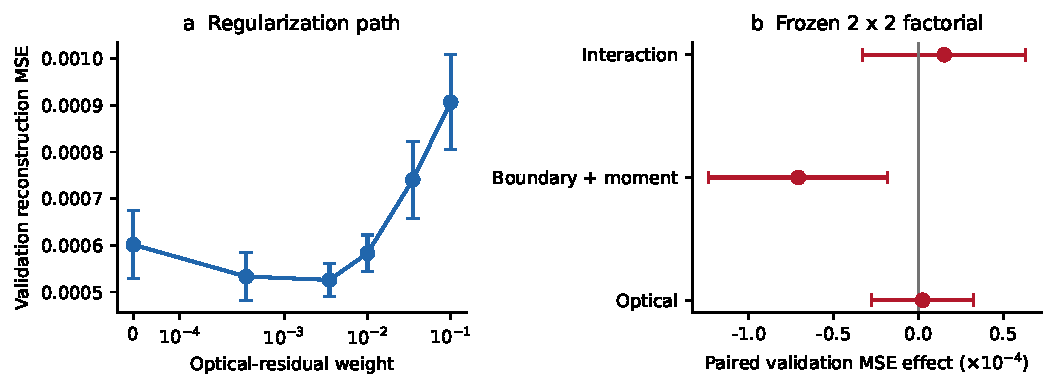
\includegraphics[width=\linewidth]{figures/figure_1_generator_mechanism.pdf}\caption{Generator mechanism diagnostics.}\end{figure}
\begin{figure}[p]
\centering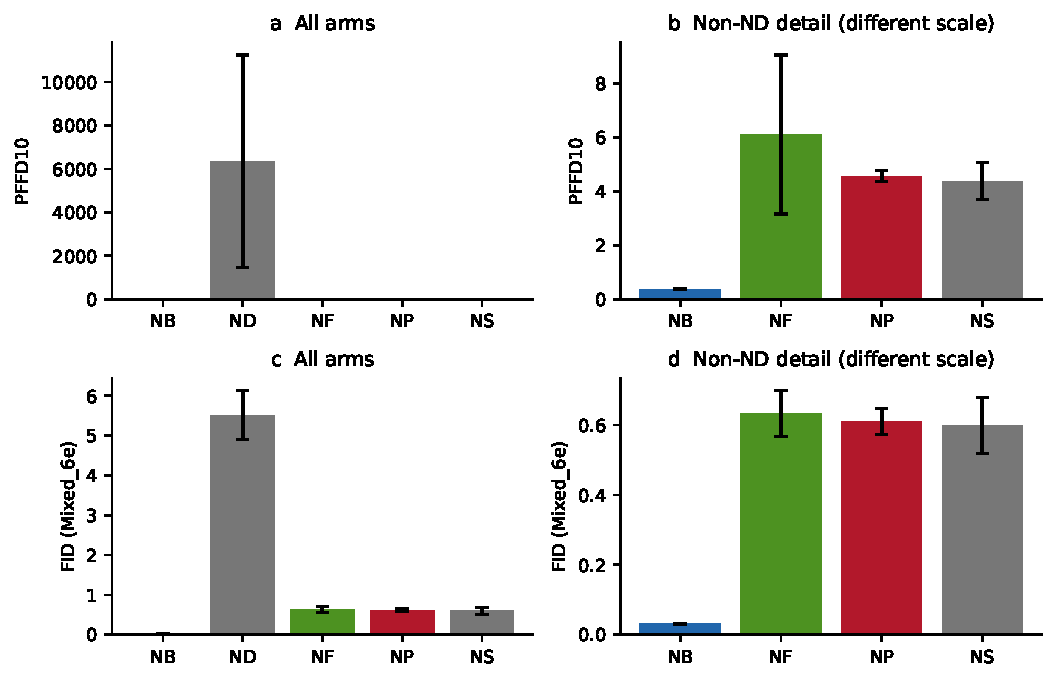
\includegraphics[width=\linewidth]{figures/figure_2_synthetic_quality.pdf}\caption{Synthetic-image quality diagnostics.}\end{figure}
\begin{figure}[p]
\centering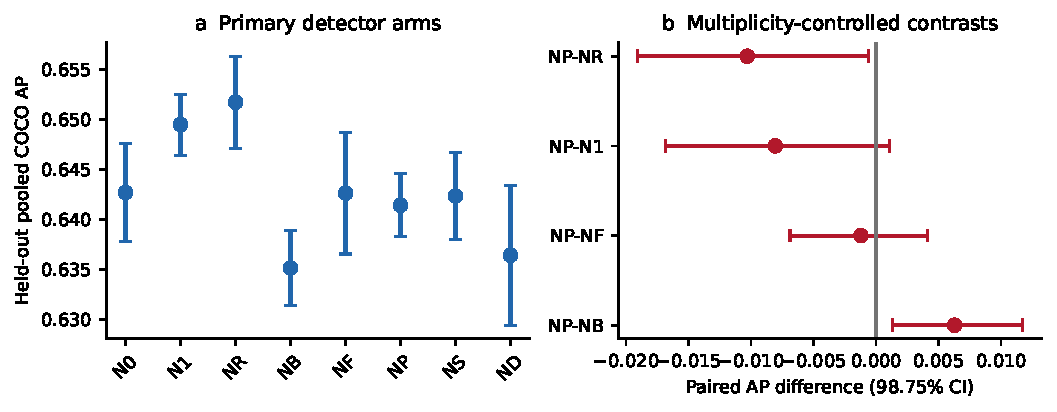
\includegraphics[width=\linewidth]{figures/figure_3_primary_detection.pdf}\caption{Frozen primary detector results.}\end{figure}
\begin{figure}[p]
\centering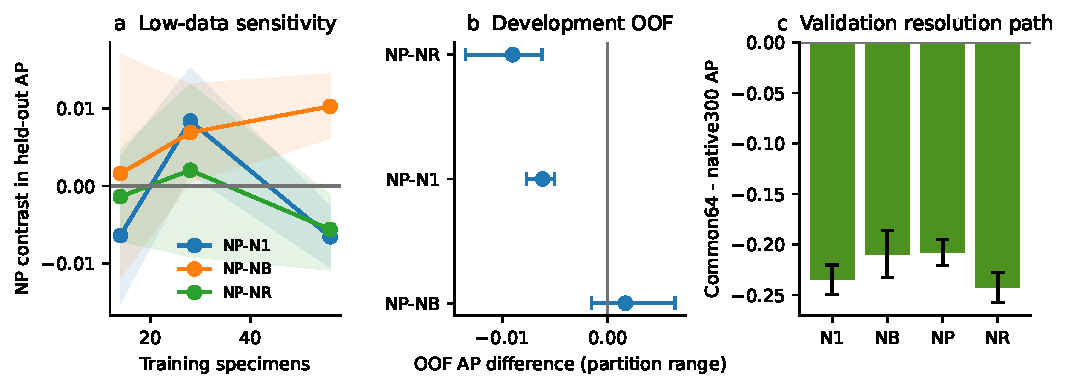
\includegraphics[width=\linewidth]{figures/figure_4_sensitivity.pdf}\caption{Secondary sensitivity analyses.}\end{figure}


\section{Discussion}
At least one predeclared multiplicity-controlled contrast separated from zero. The result supports only the observed internal operational-target comparison and does not validate the optical residual as process physics. The generator diagnostics reinforce the distinction between numerical regularization and downstream utility: the validation reconstruction path, morphology distances, and detector endpoint address different questions and need not rank methods identically. The donor-matched non-neural and additional-real-exposure arms are particularly important because gains over a weak real-only baseline can otherwise be attributed to target reuse or additional optimizer exposure.

Three limitations set the boundary of interpretation. First, the inherited box is an operational region rather than an independently adjudicated particle label; no claim is made about particle count, streak identity, or thermophysical state. Second, the 176-specimen corpus provides a specimen-grouped internal hold-out but no independent machine, build, site, material, or acquisition campaign, so external validity remains unknown. Third, the coordinate field operates at 64 pixels and the higher-resolution branch was unsupported by native information; the resolution audit quantifies a pathway effect without recovering absent detail.

Within those limits, the study contributes a falsifiable controlled evaluation rather than a physics-validity claim. Future work should obtain independently adjudicated physical targets and a prospectively acquired external cohort before using the residual or detector for process inference. A calibrated time-resolved measurement would also be required before replacing the optical operator with a governing thermal or flow residual.


\section{Methods}

\subsection{Study design and evidence layers}
The analysis separated historical evidence (H0), recovered original-code reproduction (R1), and the new frozen study (N2). Historical measurements were preserved without replacement and were not treated as targets for tuning. The N2 protocol was frozen before any N2 held-out detector outcome was accessed; this was an internal protocol freeze, not a prospective public preregistration. The same test role had been used in historical work, so the cohort was not previously unseen to the project. All development, generator-factorial, regularization, and smoothing operations used only training and validation data. A pre-unlock display of historical test identifiers was recorded as an incident; no N2 test pixel, coordinate, prediction, or metric was accessed in that event. N2 outcome evaluation began only after the pretest roster and checkpoints had been sealed.

\subsection{Dataset and operational target}
The source corpus was derived from the AI-Hub Metal 3D-Printing Spark Image Data resource (dataset 71476) \citep{aihub71476} and comprised 5,632 grayscale LPBF monitoring images from 176 specimens after the frozen study filters. Specimen identity, rather than an image or view, was the grouping unit. The frozen split assigned 112 specimens (3,584 images) to training, 32 specimens (1,024 images) to validation, and 32 specimens (1,024 images) to held-out evaluation, with views from the same specimen kept together. File-level SHA-256 digests linked each manifest row to its source image.

The inherited bounding box was treated only as an operational \texttt{inherited\_bbox\_region} target. An independent human rater study and corrected-label interaction were outside the user-approved scope. Consequently, the study does not claim human agreement, corrected-label accuracy, individual-particle segmentation, or verified physical-object semantics. Every detector conclusion is conditional on this inherited target policy.

\subsection{Conditional coordinate fields}
Images were resized to $64\times64$ pixels for coordinate-field training. A convolutional encoder mapped each image and its 13-dimensional condition vector to a 16-dimensional latent distribution. The decoder used Fourier coordinate features, a 64-unit hidden representation, and three residual blocks. Generator fits used AdamW, 10 epochs, batches of 32, 1,120 optimizer updates, paired random streams across arms, and minimum full-validation posterior-mean reconstruction mean-squared error for checkpoint selection.

The $2\times2$ factorial crossed the optical proxy term with boundary-and-moment terms across ten paired seeds. The optical weight was 0 or 0.0035; boundary and moment weights were jointly 0/0 or 0.01/0.02. A separate validation-only path used optical weights $\{0,0.00035,0.0035,0.01,0.035,0.1\}$ across three development seeds. Non-PDE controls used Gaussian scales $\{0,0.5,1,2\}$ pixels and heat-equation times $\{0,0.125,0.5,2\}$ pixel$^2$, with $\tau=\sigma^2/2$. Matching minimized the absolute relative gap in validation reconstruction error; a gap above 5\% was retained only as an unmatched diagnostic.

For intensity field $u_\theta(x,y;c,z)$ on $[-1,1]^2$, the dimensionless optical residual was
\[
r=-D(c)\nabla^2u+v_x(c)\partial_xu+v_y(c)\partial_yu+k(c)u-S(c)G(x,y;c),
\]
where $G$ is a Gaussian centred on the inherited box and coefficients are fixed functions of the condition vector, not fitted physical quantities. The objective was $L_{\rm rec}+0.0002L_{\rm KL}+w_e(\lambda_PL_P+\lambda_BL_B+\lambda_ML_M)$ with $w_e=\min(1,e/3)$ for one-based epoch $e$. Automatic differentiation evaluated the training residual at 32 random collocation points per image. $L_P$ is a detached residual-attention-weighted squared residual, $L_B$ penalizes boundary intensity, and $L_M$ penalizes intensity-squared centre and spread deviations. Supplementary Information gives every coefficient, condition normalization, and loss reduction. Validation selection used unweighted full-image MSE, not this training objective. Common finite-difference scoring and each method's own operator were kept distinct; neither is a calibrated thermal or fluid equation.

\subsection{Conditional diffusion and synthetic pools}
A compact conditional denoising model with 3.63 million parameters was trained from scratch on the same training corpus using the denoising diffusion formulation \citep{ho2020}. It used a three-scale convolutional U-Net, a cosine 1,000-step noise schedule, epsilon prediction, AdamW, batch size 16, bfloat16 automatic mixed precision, 100,000 optimizer updates per full-pipeline seed, and deterministic DDIM sampling with 50 steps and $\eta=0$ \citep{song2021}. It used no external generative pretraining.

Synthetic pools shared target conditions, training-source support, and pool size. NB, NF, NP, and NS additionally shared per-seed donor plans; ND sampled conditionally from diffusion noise rather than interpolating donors. NB blended two training images from the 64 nearest same-material/view candidates, with replacement and coefficient uniform on $[0.2,0.8]$. NF used the data-only field (F00), NP used the optical-plus-boundary/moment field (F11), and NS smoothed the boundary/moment-only field (F01) with Gaussian $\sigma=0.5$ pixels. NS is the closest unmatched control, not a successful error-matched control. Thus NP--NF is a combined-regularization contrast, not an isolated optical-term effect; the factorial isolates terms at the generator endpoint. The detector study additionally included real-only training without and with conventional augmentation (N0 and N1) and an additional-real-exposure control (NR). Synthetic boxes were inherited from the target rows rather than newly annotated; their alignment to generated content was not physically verified.

\subsection{Detector experiments}
The primary detector was Faster R-CNN \citep{ren2015} with a ResNet-50 feature pyramid backbone initialized from the checksum-verified COCO V1 weights. RetinaNet \citep{lin2017focal} with the corresponding ResNet-50 feature pyramid backbone was the secondary architecture. Inputs were $300\times300$ pixels, the effective batch size was four, bfloat16 autocast was used, and the primary checkpoint was the fixed 8,960th optimizer update. The primary matrix comprised eight arms and ten paired full-pipeline seeds. The secondary matrix comprised N1, NR, NB, and NP across five seeds. The proposed ratio grid was not run: its additional trajectories were outside the approved budget, so the preapproved fallback fixed the synthetic-to-base-real roster ratio at 0.25. Each mixed full-data roster had 3,584 base real and 896 synthetic rows (20\% synthetic presentations per complete roster pass); NR replaced those 896 rows with augmented real images. All arms received 35,840 presentations, but mixed arms had fewer real-image presentations, so equal updates did not equalize real exposure. Average precision followed the COCO intersection-over-union threshold family \citep{lin2014coco}.

Low-data experiments used three outcome-blind nested specimen subsets at 14, 28, and 56 training specimens and three pipeline seeds per subset; generators, donor banks, scalers, and detector inputs were refitted within each subset. Resolution sensitivity compared native-300 and common-64 validation inputs at fixed checkpoints. Grouped internal evaluation used three seeded three-fold partitions of the 144-specimen development cohort, nine fold-specific NP refits, and 36 detectors. Only out-of-fold predictions were scored; these folds did not provide external validation. The supplement reports all secondary architecture outcomes and the documented technical recovery of invalid RetinaNet outputs without changing checkpoints, thresholds, or seeds.

\subsection{Statistical analysis}
The primary endpoint was pooled COCO AP@[.50:.95] on held-out real images, calculated for each full-pipeline replicate and then averaged. The four primary comparisons were NP--NB, NP--NF, NP--N1, and NP--NR. Paired specimen bootstrap resampling kept views together and applied the same resampled specimen and pipeline indices to every arm. The analysis used 20,000 draws, ordinary 95\% intervals for descriptive effects, and Bonferroni-adjusted 98.75\% individual intervals for the four-comparison family. No superiority, equivalence, or non-inferiority claim was permitted solely from a confidence interval crossing zero. Historical mean-specimen AP was retained only as a secondary bridge endpoint.

Generator factorial effects were calculated within paired seeds. The optical main effect was
\[
d_s^P=\tfrac12[(F10_s-F00_s)+(F11_s-F01_s)],
\]
the boundary-and-moment main effect was
\[
d_s^{BM}=\tfrac12[(F01_s-F00_s)+(F11_s-F10_s)],
\]
and interaction was $(F11_s-F10_s)-(F01_s-F00_s)$. Failed and interrupted runs remained in the completeness and failure ledgers and were not replaced on the basis of performance.

The low-data intervals resampled the nine paired realization-by-pipeline AP differences at each subset size, conditional on the same fixed test cohort; they did not resample test specimens or model dependence from overlapping training subsets. These descriptive 95\% percentile intervals therefore do not have the primary analysis's uncertainty scope. Grouped OOF ranges span three partition-level effects and are not confidence intervals. RetinaNet results are descriptive five-seed summaries without an added confirmatory test family.

\subsection{Software, compute, and AI assistance}
All new experiments ran on a local NVIDIA GeForce RTX 5080 under the frozen software and input manifests. Run identities recorded protocol, configuration, source, environment, dataset, checkpoint, and prediction hashes. OpenAI Codex assisted with drafting and language editing, implementation and audit of experiment and analysis code, experiment orchestration, and preparation of figures and tables. Recorded programs produced the measurements; AI assistance did not substitute for measurements or author accountability. The authors must review and approve the final submitted version.

\section*{Data Availability}
The source images are governed by the AI-Hub Metal 3D-Printing Spark Image Data (dataset 71476) access and redistribution terms and are not redistributed in the public reproducibility package. Split-level cohort metadata, derived numerical evidence, figure source data, and aggregate reconstruction instructions are available at \ReleaseURL. The public package excludes licensed source pixels and disallowed path-level provenance.

\section*{Code availability}
The custom study runners, statistical, and package-verification code are available at \ReleaseURL in release \ReleaseVersion, with SHA-256 checksums. The public route rebuilds aggregate text, tables, and figures. Full retraining and raw-prediction bootstrap reproduction additionally require authorized images, excluded recovered historical source dependencies, and prediction payloads; the public archive alone is not a turnkey full-experiment environment.

\bibliographystyle{unsrtnat}
\bibliography{references}

\section*{Acknowledgements}
This work was supported by the Institute of Information \& Communications Technology Planning \& Evaluation (IITP) Innovative Human Resource Development for Local Intellectualization program grant funded by the Korea government (MSIT) (IITP-2026-RS-2024-00436773). \authoraction{Confirm funder wording and grant number.}

\section*{Author contributions}
The working contribution record assigns software, validation, visualization, and preparation of the original draft to H.P.; supervision, resources, and review and editing to N.-H.Y.; and conceptualization, methodology, supervision, project administration, funding acquisition, and review and editing to J.Y. \authoraction{Each author must confirm or correct these roles and approve the final manuscript before submission.}

\section*{Competing interests}
\authoraction{Insert the competing-interest declaration confirmed by every author. The working record currently indicates no competing interests, but this has not been attested and must not be submitted as fact until confirmed.}

\section*{Figure legends}
\textbf{Figure 1. Generator mechanism diagnostics.} (a) Validation reconstruction MSE across the frozen optical-weight path (mean and standard deviation over three seeds). (b) Paired $2\times2$ factorial effects with 95\% Student-$t$ intervals over ten seeds. Lower MSE is better; neither panel uses held-out test outcomes.\par
\textbf{Figure 2. Synthetic-image quality diagnostics.} Mean and standard deviation over ten paired seeds for (a) the training-scaled ten-feature morphology Fr\'echet distance (PFFD10) and (b) Fr\'echet distance in ImageNet Inception-v3 Mixed\_6e features. Lower values indicate closer aggregate distributions but are not measures of physical validity.\par
\textbf{Figure 3. Frozen primary detector results.} (a) Mean and standard deviation of held-out pooled COCO AP@[.50:.95] across ten full-pipeline replicates. (b) Four paired primary contrasts with Bonferroni-adjusted 98.75\% individual bootstrap intervals. Positive values favour NP.\par
\textbf{Figure 4. Secondary sensitivity analyses.} (a) Low-data held-out effects with ordinary 95\% intervals. (b) Grouped out-of-fold development-cohort effects with ranges across three partition seeds. (c) Validation AP change after the common-64 information pathway relative to native-300 evaluation.


\end{document}
